\documentclass[11pt, a4paper]{article}
\usepackage[paper=a4paper, left=1.5cm, right=1.5cm, bottom=1.5cm, top=1.5cm]{geometry}
\usepackage[utf8]{inputenc}
\usepackage{clrscode3e}
\usepackage[spanish]{babel}
\newcommand\Frac[3][]{ #1 #2\color{black}\above 0.4pt \normalcolor #1#3}
\usepackage{amsmath,amssymb}
\usepackage{xcolor}
\usepackage{caratula/caratula}
\usepackage{bm}

\usepackage{listings}
\usepackage{color}
 
\definecolor{codegreen}{rgb}{0,0.6,0}
\definecolor{codegray}{rgb}{0.5,0.5,0.5}
\definecolor{codepurple}{rgb}{0.58,0,0.82}
\definecolor{backcolour}{rgb}{0.95,0.95,0.92}
 
\lstdefinestyle{coding}{
    backgroundcolor=\color{backcolour},   
    commentstyle=\color{codegreen},
    keywordstyle=\color{magenta},
    numberstyle=\tiny\color{codegray},
    stringstyle=\color{codepurple},
    basicstyle=\footnotesize,
    breakatwhitespace=false,         
    breaklines=true,                 
    captionpos=b,                    
    keepspaces=true,                 
    numbers=left,                    
    numbersep=5pt,                  
    showspaces=false,                
    showstringspaces=false,
    showtabs=false,                  
    tabsize=1
}
 
\lstset{literate=%
{$}{{\$}}1
{å}{{\aa}}1
{ø}{{\o}}1
{Æ}{{\AE}}1
{Å}{{\AA}}1
{Ø}{{\O}}1
}
\lstset{extendedchars=\true}
\lstset{inputencoding=ansinew}
 
 
\lstset{style=coding}

\begin{document}

\titulo{Trabajo Práctico 1 }
\fecha{Domingo 16 de Septiembre de 2018}
\materia{Algoritmos y Estructuras de Datos III}

\integrante{Kennedy Williams Rios Cuba}{381/15}{wrios@dc.uba.ar}

%Carátula
\maketitle
\newpage

%Indice
\tableofcontents
\newpage

%Introduccion
\section{Introducción al Problema}

\subsection{Definici\'on del problema Subset Sum}
Dado un conjunto de n \'items $S$, cada uno con un $valor$ asociado $v_{i}$ , y un valor objetivo $V$ ,
decidir si existe un subconjunto de \'items de S que sumen exacto el valor objetivo $V$ . Si existe
dicho conjunto, decir cual es la m\'inima cardinalidad
P entre todos los subconjuntos posibles. \\
En otras palabras decidir si existe$ R \subseteq S$ tal que $\sum_{i \in R}v_{i} = V$, y si existe, devolver la menor cardinalidad posible de $R$.\\
Para este problema, asumiremos que todos los valores mencionados son enteros no negativos.
\subsection{Ejemplo de problema}

\subsubsection{Ejemplo 1}
En este ejemplo se puede ver cual es el espacio de soluciones, la forma de recorrerlo será
definida más adelante  de acuerdo a cada algoritmo que usemos para resolver el problema.
Además se ver\'a que tamaño tiene este espacio, y la cantidad de posibles soluciones (en el diagrama se logra ver como cada nodo hoja es una posible soluci\'on que llego desde las decisiones tomadas).\\
Se considera un conjunto de 4 elementos $\{11,7,5,2\}$.\\
Se busca que la suma de los elementos sea 18 y que el cardinal sea mínimo.\\
El nivel i representa la decisión de tomar el elemento (con un + arriba del nodo) o no
tomar el elemento (con un - arriba del nodo) para mirar si forma parte de la solución.
Como se puede ver en el gráfico, hay dos soluciones $\{11,7\}$ y $\{11,5,2\}$ que suman 18 pero
la mejor es usando menos elementos, con lo cual nos quedamos con la solución $\{11,7\}$.
\begin{center}
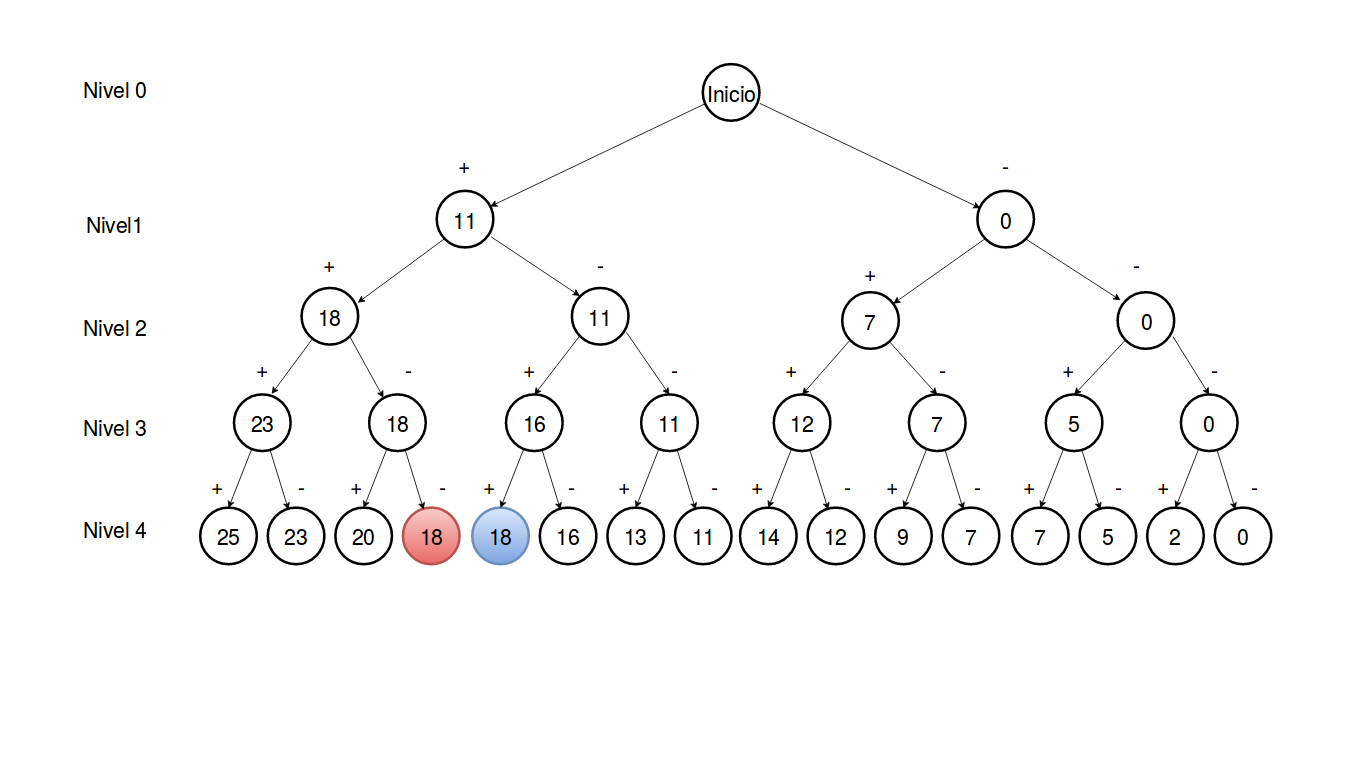
\includegraphics[width=18cm, height=12cm]{diagrama.png}
\end{center}
\subsubsection{Ejemplo 2}
Conjunto $\{2, 3, 12, 14, 4\}$, buscamos un subconjunto de elementos que sume 13.\\
El 14, no puede sumar 13. El 12 no se puede elegir porque no hay elementos que sumen 1. Al combinar cualquiera de los que restan, no alcanzan a sumar 13 con lo cual no hay soluci\'on para este problema.\\


\subsection{El objetivo del trabajo pr\'actico}
 Resolver el problema propuesto de diferentes maneras realizando posteriormente una comparaci\'on entre los diferentes algoritmos utilizados.
%\newpage

%Desarrollo
\section{Desarrollo Problema}
\subsection{Caracterizaci\'on de una soluci\'on}
\begin{itemize}
	\item Una posible soluci\'on es un subconjunto de elementos del conjunto original tal que la suma de ellos es menor al valor objetivo.
	\item Una soluci\'on factible de nuestro problema es un subconjunto de elementos del conjunto original tal que la suma de ellos es exactamente el valor objetivo.
	\item Una soluci\'on no factible es un subconjunto de elementos del conjunto original tal que la suma de ellos es mayor al valor objetivo
\end{itemize}
\subsection{Espacio de soluciones}
En la imagen podemos ver, que luego de diferentes decisiones, llegamos a diferentes soluciones.
\begin{itemize}
	\item Los nodos hojas son las soluciones y est\'an separados en tres casos.
	\item Los nodos celestes son las posibles soluciones.
	\item Los nodos verdes son las soluciones factibles.
	\item Los nodos rojos son las soluciones no factibles. 
\end{itemize}	
\begin{center}
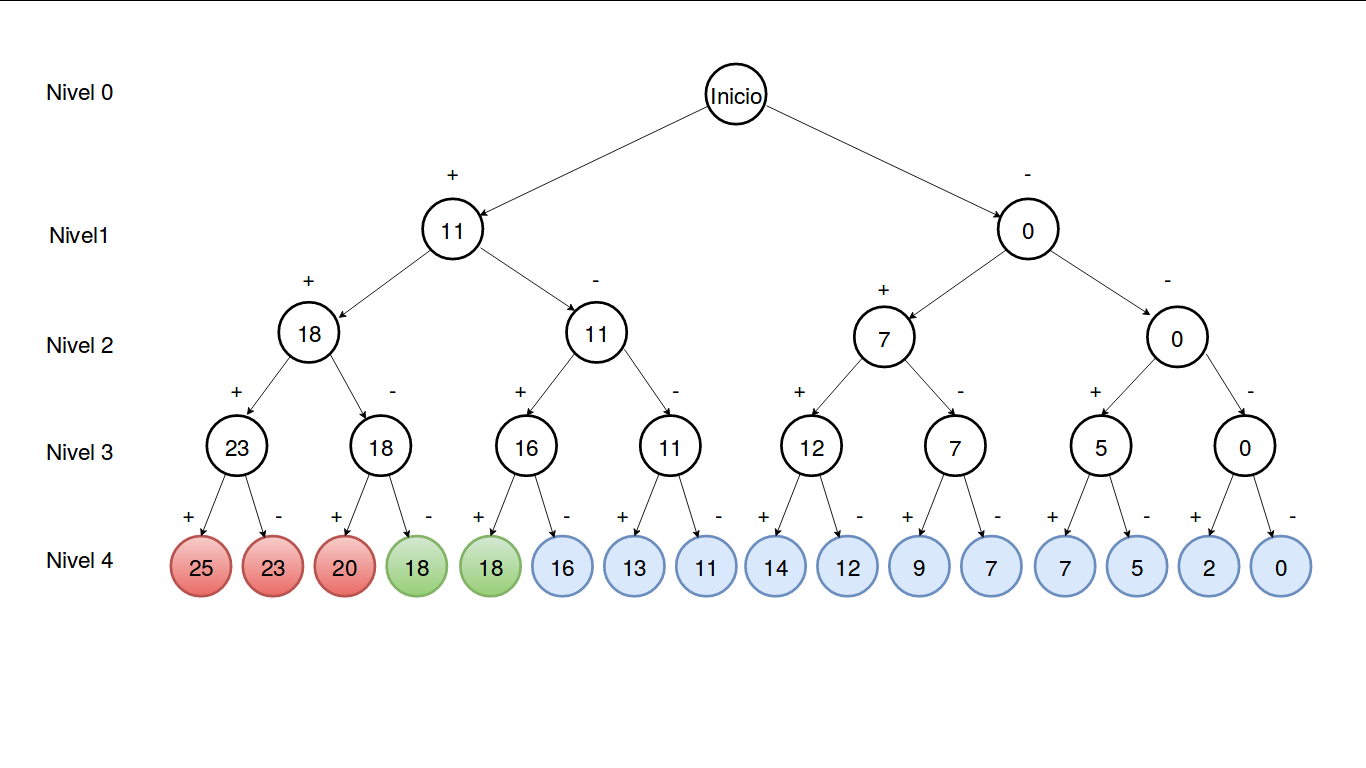
\includegraphics[width=18cm, height=12cm]{3casos.png}
\end{center}
\subsection{Recorrido del espacio de soluciones}
Se ver\'an diferentes formas de pensar el problema, y en base a ello elegiremos una forma de obtener la soluci\'on.\\

\begin{itemize}
\item La primer forma de ver el problema es simple, mirar todo el espacio de soluciones y quedarnos con la mejor.\\
\item En la segunda forma trataremos de recorrer solamente el espacio de posibles soluciones y el espacio de soluciones factibles.\\
\item La tercer forma va mas enfocado a cuando una soluci\'on es mejor que otra, y veremos como recorrer las soluciones que son mejores que la soluci\'on que tenemos hasta el momento(si las hay, sino podaremos).\\
\item La ultima forma de pensar el problema sera ver los problemas anteriores inmediatos y ver como con ellos se puede construir el problema mas grande y gracias a memorizar los subproblemas poder obtener el siguiente de forma eficiente.
\end{itemize}

%Fuerza Fruta
\section{Fuerza Bruta: Recorriendo todo el espacio}
\subsection{Algoritmo}


\begin{codebox}
    \Procname{\proc{FB}(S, int V, int i, int n) \quad\quad\textcolor{green}{O($2^n$)}}
    \li \If $i <= n:$ \quad\quad\textcolor{green}{O($1$)}
        \Then
    \li   
            \Return $min(1+FB(S,V-C_{i},i+1,n),FB(S,V,i+1,n))$
        \End
    \li \If $V = 0:$ \quad\quad\textcolor{green}{O($1$)}
        \Then
    \li        
            \Return $0$
        \End
    \li     \Return $\infinity$

    \end{codebox}

\begin{codebox}
    \Procname{\proc{ResolverFB}(S, int V, int i, int n) \quad\quad\textcolor{green}{O($2^n$)}}
    \li $sol \leftarrow FB(S,V,i+1,n)$
    \li \If $sol = \infinity:$ \quad\quad\textcolor{green}{O($1$)}
        \Then
    \li   
            \Return $-1$
        \End
    \li     \Return $sol$

    \end{codebox}    
\subsection{Correctitud}
El algoritmo recorre todo el espacio de busqueda, lo \'unico que hace es guardar la mejor soluci\'on hasta el momento, y luego devuelve la soluci\'on que tiene o -1 si no encontr\'o soluci\'on.\\
El algoritmo es correcto pues recorre todo el espacio de soluciones y solamente conserva las soluciones v\'alidas y se queda con la mejor.
\subsection{Complejidad}
El algoritmo se divide en dos casos, donde se llama recursivamente con un elemento menos.\\
Definiendo la siguiente ecuaci\'on de recurrencia:\\
$$
T(n) = \left\{
\begin{array}{cl}
 \Theta (1) &\mbox{si
} n = 1 \\
2T(n)+1&\mbox{si } n > 1
\end{array}\right.
$$
\\
Como podemos ver, la recurrencia:\\ $T(n)= 2T(n-1) + 1 = 2(2T(n-1)+1)+1= ...= 2^{n-1}+ (n-1) = O(2^{n})$.\\
Con lo cual tiene complejidad: $O(2^{n})$.\\
%\newpage

%Backtracking
\section{Backtracking: Fuerza Bruta Inteligente}
\subsection{Factibilidad: recorrido siempre v\'alido}
Una camino en el \'arbol del espacio de soluciones, es v\'alido, siempre y cuando la suma de sus elementos no exceda el valor objetivo.
Con esto en mente, si encontramos un camino para el cual la suma de sus elementos es mayor al valor objetivo, al estar trabajando con enteros positivos, si seguimos agregando elementos la suma siempre exceder\'a el valor objetivo, por lo tanto cortamos esa rama del espacio de soluciones y seguimos por otra rama.\\

\subsubsection{Algoritmo}
\begin{codebox}
    \Procname{\proc{Fac}($S$, $int$ $V$, $int$ $i$, $int$ $n$)\quad\quad\textcolor{green}{O($2^n$)}}
    \li \If $i \leq n:$\quad\quad\textcolor{green}{O($1$)}
        \Then
    \li     \If $V-S_{i} > 0:$\quad\quad\textcolor{green}{O($1$)}
                \Then
    \li              \Return $min(Fac(S,V,i+1,n),1 +Fac(S, V-S_{i}, i+1, n))$
                \End         
    \li     \If $V = 0 :$\quad\quad\textcolor{green}{O($1$)}
                \Then
    \li             \Return $0$
                \End
            \End
    \li \Return $\infinity$ 

    \end{codebox}

\begin{codebox}
    \Procname{\proc{ResolverFac}(S, int V, int i, int n) \quad\quad\textcolor{green}{O($2^n$)}}
    \li $sol \leftarrow Fac(S,V,i+1,n)$
    \li \If $sol = \infinity:$ \quad\quad\textcolor{green}{O($1$)}
        \Then
    \li   
            \Return $-1$
        \End
    \li     \Return $sol$

    \end{codebox}        
\subsubsection{Correctitud}
El algoritmo recorre solomente las ramas que tienen soluci\'on, con lo cual, llega a las mismas soluciones que Fuerza Bruta y lo \'unico que hace es quedarse con la mejor soluci\'on.
\subsubsection{Complejidad}
Vemos que el algoritmo define la misma recurrencia que fuerza bruta:\\
$$
T(n) = \left\{
\begin{array}{cl}
 \Theta (1) &\mbox{si
} n = 1 \\
2T(n)+1&\mbox{si } n > 1
\end{array}\right.
$$
\\
Con lo cual tiene complejidad en peor caso: $O(2^{n})$.\\
\subsection{Optimalidad: Recorrido siempre \'optimo}
Para nuestro problema, una soluci\'on es \'optima, si la cantidad de elementos de la soluci\'on es menor o igual que la cantidad de elementos para toda otra soluci\'on.\\
Dado una rama del espacio de b\'usqueda definido por el recorrido, si la cantidad de elementos de la rama es mayor o igual a la cantidad de elementos de la mejor soluci\'on encontrada hasta el momento, entonces se poda esa rama.\\
La poda solo corta las ramas con mayor o igual cantidad de elementos que pueden o no llegar a una soluci\'on\\
\subsubsection{Algoritmo}
\begin{codebox}
    \Procname{\proc{Op}($S$, $int$ $V$, $int$ $i$, $int$ $n$, $int$ $cantidad$, $int$ $optActual$) \textcolor{green}{O($2^n$)}}
    \li \If $i \leq n:$\quad\quad\textcolor{green}{O($1$)}
            \Then
    \li        \If $ cantidad < optActual:$
                \Then
                \li $optActual \leftarrow cantidad$
    \li             \Return $min(Op(S,V,i+1,n,cantidad,optActual),1 + Op(S, V-C_{i}, i+1, n, cantidad, optActual))$
            \End
    \li        \If $V = 0:$
                \Then
    \li             \Return $0$
            \End
        \End
    \li \Return $\infinity$

    \end{codebox}
    \begin{codebox}
    \Procname{\proc{ResolverOp}(S, int V, int i, int n) \quad\quad\textcolor{green}{O($2^n$)}}
    \li $sol \leftarrow Op(S,V,i+1,n)$
    \li \If $sol = \infinity:$ \quad\quad\textcolor{green}{O($1$)}
        \Then
    \li   
            \Return $-1$
        \End
    \li     \Return $sol$

    \end{codebox}    
\subsubsection{Correctitud}
Supongamos que existe soluci\'on y el algoritmo no encuentra, el algoritmo no poda (hace Fuerza Bruta) hasta encontrar una soluci\'on, como no encuentra soluci\'on Fuerza Bruta no encuentra soluci\'on. \\
Absurdo pues Fuerza Bruta explora todo el espacio de soluciones.\\
Por lo tanto, si hay soluci\'on la encuentra.\\
Supongamos que hay una soluci\'on \'optima $S$ de cardinal $k$ y el algoritmo no lo encuentra:\\
Sea$ n = |S'|$ ($S'$ la soluci\'on retornada con cardinal $n$ y $n > k$), entonces antes de encontrar a $S'$, no hab\'ia soluci\'on o la anterior soluci\'on tenia mayor cardinal.\\

\begin{itemize}
	\item Caso Sin Soluci\'on anterior: El algoritmo poda toda soluci\'on de cardinal $>= n$.
	\item Caso Hab\'ia Soluci\'on anterior: Sea $m$ el cardinal de la soluci\'on anterior, sabemos que $n < m$.\\
	Se podaron las soluciones $>= m$, en particular no se podo ninguna soluci\'on con cardinal $< n$.\\
\end{itemize}	
Absurdo pues $k < n$ con lo cual $S$ fue podado.
Entonces si existe una soluci\'on \'optima, el algoritmo lo encuentra y lo devuelve.
\subsubsection{Complejidad}
Vemos que algoritmo define la misma recurrencia que fuerza bruta:\\
$$
T(n) = \left\{
\begin{array}{cl}
 \Theta (1) &\mbox{si
} n = 1 \\
2T(n)+1&\mbox{si } n > 1
\end{array}\right.
$$
\\
Con lo cual tiene complejidad en peor caso: $O(2^{n})$.\\
%\newpage


%Dinámica
\section{Programación Dinámica: Colision y Memoizacion}
\subsection{principio del Optimalidad: para Subset Sum}
Sea $S1$ la solucion optima usando $X_{1},...,X_{n-1}$, tal que sumen $V-X_{n}$\\
Sea $S2$ la solucion optima usando $X_{1},...,X_{n-1}$, tal que sumen $V$\\
Sea S = min(S1, S2), la solucion optima para el problema de n-elementos, entonces hay 2 opciones:\\
Usar el n-esimo elementos, o no usarlo.\\
Supongamos que $S$ no es solucion optima, como S no es optimo entonces existe S' tal que |S'|<|S|.\\
\begin{itemize}
    \item Caso $X_{n}$ pertenece a $S$: $|S'| < |S| = |S1|+1$, entonces $|S'|-1 < |S1|$, como $S1$ es el optimo para sumar $V-X_{n}$ usando $X_{1},...,X_{n-1}$ y $|S'-X_{n}|$ es un conjunto de elementos que suman $V-X_{n}$ y es menor que el optimo. Absurdo pues $S1$ es optimo.
    \item Caso $X_{n}$ no pertenece a $S$: $|S'| < |S| = |S2|$. Absurdo pues $S2$ es el optimo para sumar V usando $X_{1},...,X_{n-1}$ 
\end{itemize}
Vimos en la introducci\'on que las soluciones de este problema pueden ser expresados mediante una secuencia de decisiones.\\
Ahora para que ver cumple el principio de optimalidad definimos:

 \begin{equation}
     \label{eq:F-recursiva}
     F(x) = \left\{
	       \begin{array}{ll}
		 0      & \mathrm{si\ }  C = \{\} \hspace{4mm} y\hspace{4mm} S = 0\\
		 min(1+F(C-V_{n},S-valor(V_{n})),F(C-V_{n},S)) & \mathrm{si\ } n > 1 \\
		 \infty     & \mathrm{si\ } C = \{\} \hspace{4mm} y \hspace{4mm} S < 0
	       \end{array}
	     \right.
   \end{equation}
Llamamos al problema \'optimo de resolver el problema original con un elemento menos(usando el n-esimo elemento y sin usar el n-esimo elemento que son los dos \'unicos casos), osea dos subproblemas \'optimos. Por lo tanto con esos dos subproblemas se puede armar el problema mas grande.\\
Con lo cual, podemos usar Programaci\'on din\'amica para resolver el problema.

\subsection{Algoritmo}
\begin{codebox}
    \Procname{\proc{FB}(vec$\<$int$\>$ C, int V, int i, int n) \textcolor{red}{O($2^n$)}}
    \li \If $i <= n$ \quad\quad\quad\quad\quad\quad\quad\textcolor{red}{O($1$)}
        \Then
    \li        \If $V == 0$ : \quad\quad\quad\quad\quad\quad\textcolor{red}{O($1$)}
                \Then
    \li             \Return $0$ \quad\quad\quad\quad\quad\quad\quad\textcolor{red}{O($1$)}
    \li         \Else: 
    \li                 \Return $Inf$\footnote{Si el algor\'itmo devulve un n\'umero mayor que $n$ significa que no existe soluci\'on} \quad\quad\quad\quad\quad\quad\quad\textcolor{red}{O($1$)}
                \End
                \End

    \li \Return min(FB($C$,$V$,$i+1$,$n$),$1 +$FB($C$, $V-C_{i}$, $i+1$, $n$)) \textcolor{red}{O($2^n$)}

    \end{codebox}
\subsection{Correctitud}
Dado que subset-sum cumple el principio de optimalidad, se puede usar esa forma recursiva para poder calcular el valor optimo.\\
Ahora veremos que el algoritmo devuelve lo mismo que la funcion.\\
\subsection{Complejidad}
La complejidad es f\'acil de deducir, se recorren dos array de cardinal V y se llama a la iteraci\'on n veces.\\
Por lo tanto la complejidad es O(V*n)


%Experimentación
\section{Experimentación}
\subsection{Hipotesis}
\begin{itemize}
	\item Las podas de factibilidad y optimalidad en mejor caso tienen complejidad lineal.
	\item Hacer un sort de los elementos de mayor a menor, hace que las podas sean m\'as efectivas.
	\item Hacer un sort de los elementos de menor a mayor, hace que las podas empeoren y sean mas parecidas a fuerza bruta
	\item La poda de factibilidad empeora a medida que el valor de los elementos se acercan a 0, y mejora a medida que el valor de los elementos se acercan al valor objetivo
	\item Fuerza Bruta depende unicamente de la cantida de items
\end{itemize}
\subsection{Consideraciones para las experimentaciones}
\subsubsection{Generaci\'on de elementos}
\begin{itemize}
	\item Se usa la funcion sort de c++ (ordena los elementos en forma creciente)
	\item Los conjuntos fueron generados aleatoriamente, con la funci\'on rand de c++ (distribucion uniforme) para poder analizar en caso promedio que pasaba con cada algoritmo, en el rango entre [0..V].
	\item la cantidad de iteracione es igual a 50, pues se logro ver durante la experimentaci\'on que los algoritmos se estabilizaban.
	\item El rango para la suma fue [15000...80000], porque es limitada por Programacion Dinamica, la cual pide memoria de tamaño n*W y al ser W tan grande, hace que no se pueda seguir experimentando.
	\item El rango para la cantidad de elementos fue [5...35], porque al querer analizar el caso promedio se toma el promedio de 50 iteraciones y los algoritmos exponenciales tard\'an demasiado.
\end{itemize}
\subsubsection{Im\'agenes y Complejidades}
\begin{itemize}
	\item Para medir el tiempo se tomó el promedio 50 de iteraciones
	\item Para todos los algoritmos se grafica el tiempo en el eje Y (en ns), y la cantidad de elementos en el eje X
	\item Para todos los algoritmos se dan 2 gr\'aficos, el primero es como crece en funci\'on de la cantidad de elementos, luego el segundo algoritmo dividido por su complejidad te\'orica
	\item Todos los gr\'aficos con excepci\'on del \'ultimo fueron hecho con la suma objetivo igual a 500(el ultimo gr\'afico no, para poder mostrar como afecta el valor de la suma al algoritmo de Programaci\'on din\'amica)
\end{itemize}	
\subsection{Complejidades Te\'oricas en la practica}
\subsubsection{Fuerza Bruta}
Fuerza Bruta no es afectada por el sort de los elemento, y al aplicarle el logaritmo en base dos se logra ver que es lineal, lo cual es esperado pues es exponencial en la cantidad de elementos con base igual a 2.
\begin{center}
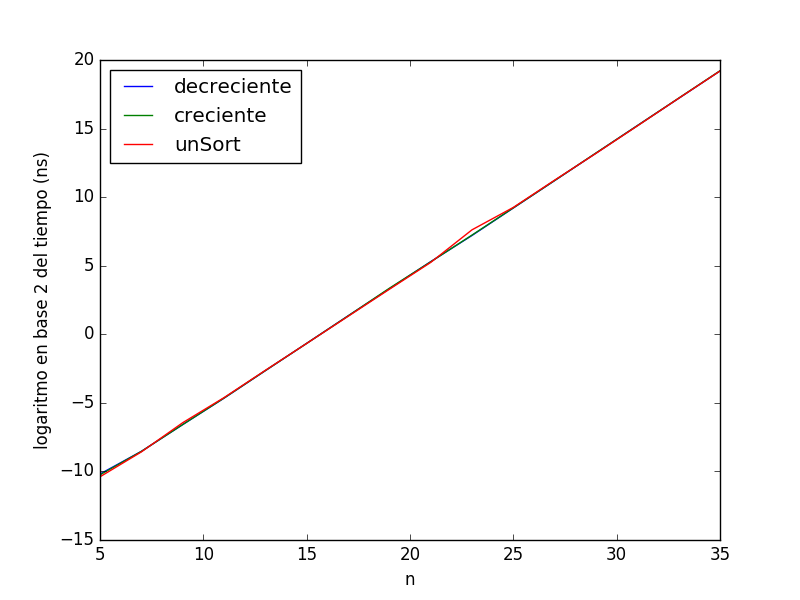
\includegraphics[width=16cm, height=11cm]{fbSort.png}
\end{center}

\subsubsection{Backtracking poda por factibilidad}
Tener los elementos ordenados de mayor a menor hace que la poda sea mas efectiva y empeora cuando el ordenamiento es de menor a mayor.\\
Se aplica logaritmo en base dos y se logra ver que el resultado es lineal.
\begin{center}
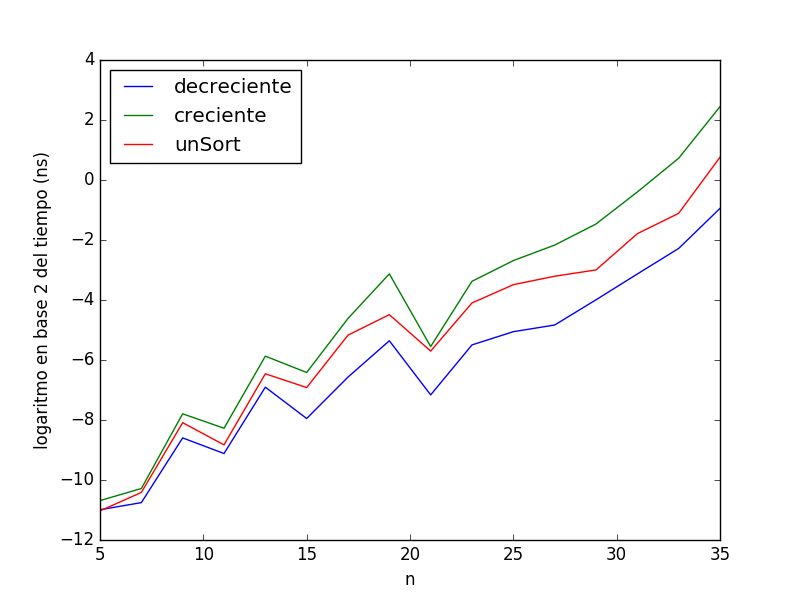
\includegraphics[width=16cm, height=11cm]{facSort.png}
\end{center}
\subsubsection{Backtracking poda por optimalidad}
El ordenamiento de los elementos afecta a la poda de optimalidad y se hace el mismo analisis que para la poda de factibilidad.
\begin{center}
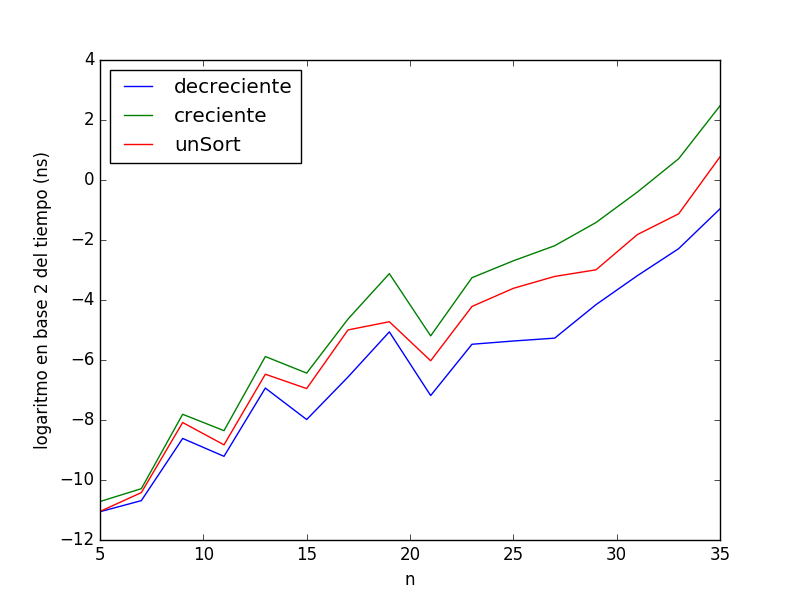
\includegraphics[width=16cm, height=11cm]{opSort.png}
\end{center}
\subsubsection{Programacion dinamica}
Para esta experimentacion se varia V y se compara el tiempo en funcion de el ordenamiento de los elementos.\\
El resultado es el esperado pues, en el grafico se ve como Programacion Dinamica es afectado directamente por el valor objetivo.
\begin{center}
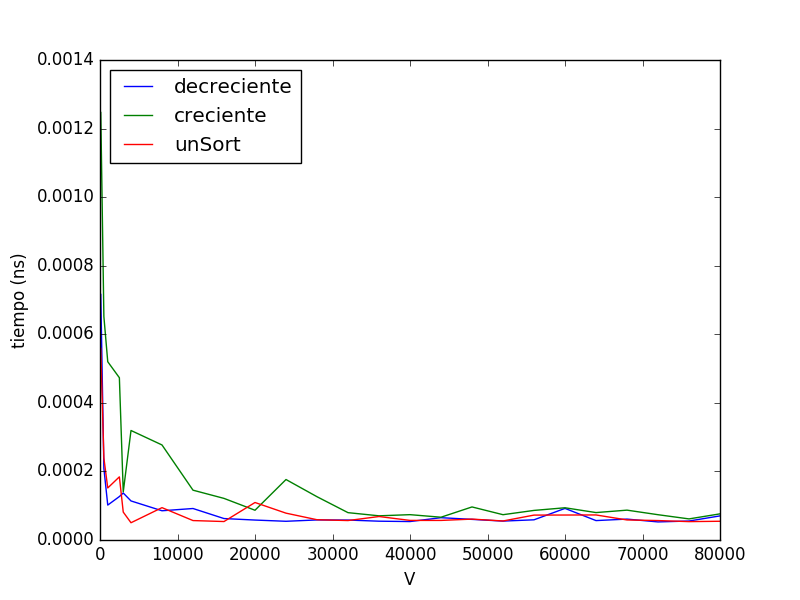
\includegraphics[width=16cm, height=11cm]{pdSuma.png}
\end{center}
%\begin{center}
%\includegraphics[width=16cm, height=11cm]{todosFac_objetivos_90000.png}
%\end{center}
%\newpage

%Conclusión
\section{Conclusión}
Se llego a ver que las podas y Programación dinámica son afectados por el sort de los elementos, y el valor de ellos.
También que Programación dinámica es mas afectada por el valor objetivo, que por el sort de los elementos.\\
Fuerza Bruta depende únicamente de la cantidad de items.\\
La figura 5 muestra que a medida que el valor de los elementos es mas chico, las podas empeoran y se parecen cada vez mas a Fuerza Bruta.\\
Para resolver este problema, Programación dinámica es el mejor de los 4 algoritmos si el valor objetivo es lo suficientemente chico para poder usarla. En cambio sí no lo es, se usaría Backtracking teniendo en cuenta el valor de los elementos y el previo ordenamiento de los mismos.\\
%\newpage

\end{document}
